\subsection{Models}

The train set used for this phase of exploring various classifiers consists mainly of four datasets: unigrams and bigrams, embeddings, stylistic features, and the offensiveness score. Depending on which embeddings dataset is used the dimensionality may change, but in general it is around 7000 total features.
{}
After tuning the hyperparemeters of several classifiers (Logistic Regression, SVM, Random Forest, XGBoost, Light-GBM) the best one turned out to be Light-GBM (with an average F1-macro of 0.774 on 5 folds of cross-validation), as well as being clearly the fastest. Thus, we used this first version of the model to carry out several analyses regarding features.
For example, with respect to feature importance: although any of the four datasets manages, taken individually for training, to achieve an average F1-macro of at least 0.75, when used all together the model takes into account almost only the embeddings to classify (and a few other interesting features such as the unigrams 'rom' and 'terrorism', the stylistic features 'uppercase\_words\_dist' and 'lexical\_density', and 'offensiveness\_score' and 'badword').
Moreover, thanks to the calculation of feature importance, we were able to observe that the model does not benefit at all from many of our features, as it achieves its highest result (average F1-macro of 0.784) using only the first 100, as shown by the plot at figure \ref{fig:features}.

\begin{figure}
    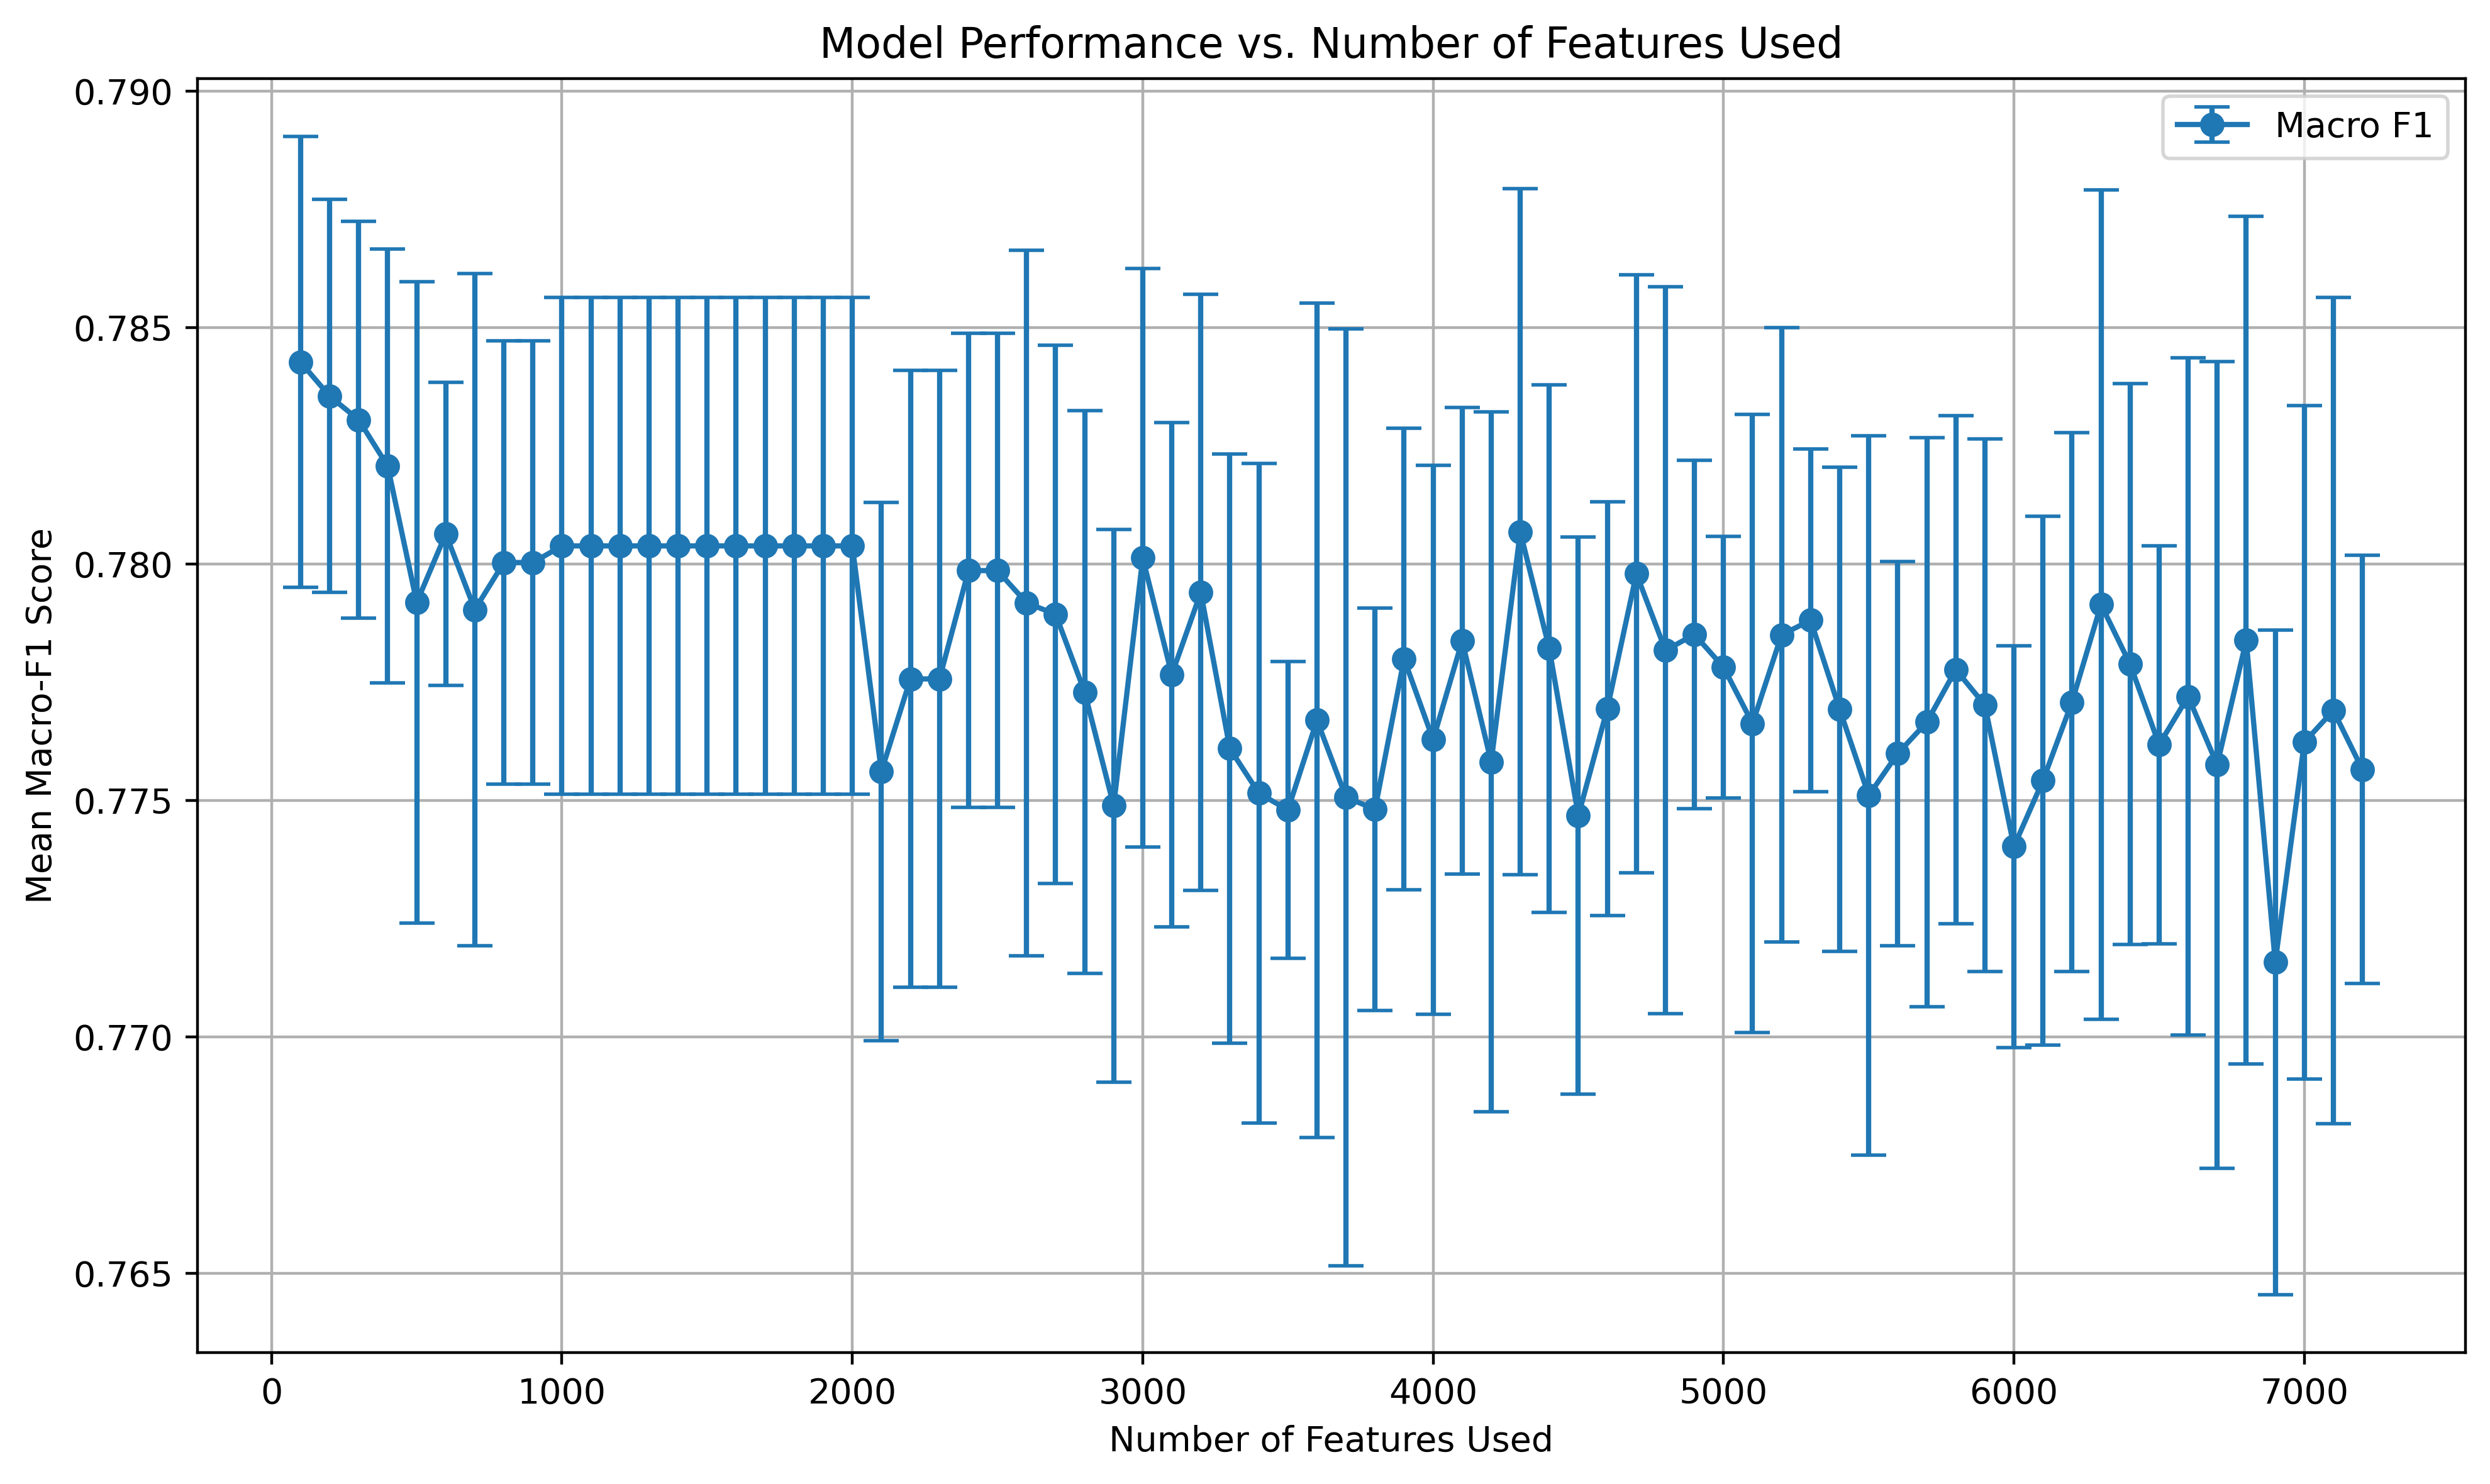
\includegraphics[width=\columnwidth]{../../results/images/model_n_feats.png}
    \caption{Performance of LGBM classifier vs number of features used by the classifier}
    \label{fig:features}
\end{figure}
Regarding embeddings, since they are apparently the most useful feature set, we trained the model on all the embeddings datasets we computed to check if there is any noticeable difference, and we found that the one that best performing embeddings are the mean pooled embeddings from AlBERTo.

With regard to the offensiveness score, we found instead that the score normalized by the length of the tweet returned better results than the non-normalized score and than both scores used together.

Finally, after all the information obtained, we performed a more comprehensive randomized search to re-tune the hyperparameters of the Light-GBM in order to have a definitive model to use for testing (the model reached an average F1-macro of 0.778 on the validation set). For the generalisation task, since the stylistic features are very different between tweets and newspaper headlines, we decided to perform a second tuning to generate another model that is not trained on stylistic features.